\section{Durchführung}
\label{sec:Durchführung}

\subsection{Elementare Komponenten für den Versuch}
\label{sec:d1}
Neben dem Szintillator sind noch einige weitere Komponenten wichtig für die 
erfolgreiche Durchführung des Experiments. Dazu gehören zum Einen die Photomultiplier.
diese sind darauf ausgelegt, auch schwache Lichstignale zu messen. Trifft ein 
Photon auf die Photokathode, so werden Elektronen über den photoelektrischen
Effekt rausgelöst. Sie werden durch ein elektrisches Feld beschleunigt und 
treffen auf eine Kette von Dynoden, sodass sich die Elektronenzahl bei jedem 
Aufprall auf eine Dynode vervielfacht. Am Ende kann das Signal durch einen 
Spannungsabfall an einem Widerstand gemessen werden. Der schematische Plan 
ist in \autoref{fig:d1} abgebildet. 
\begin{figure}[H]
    \centering
        \centering
        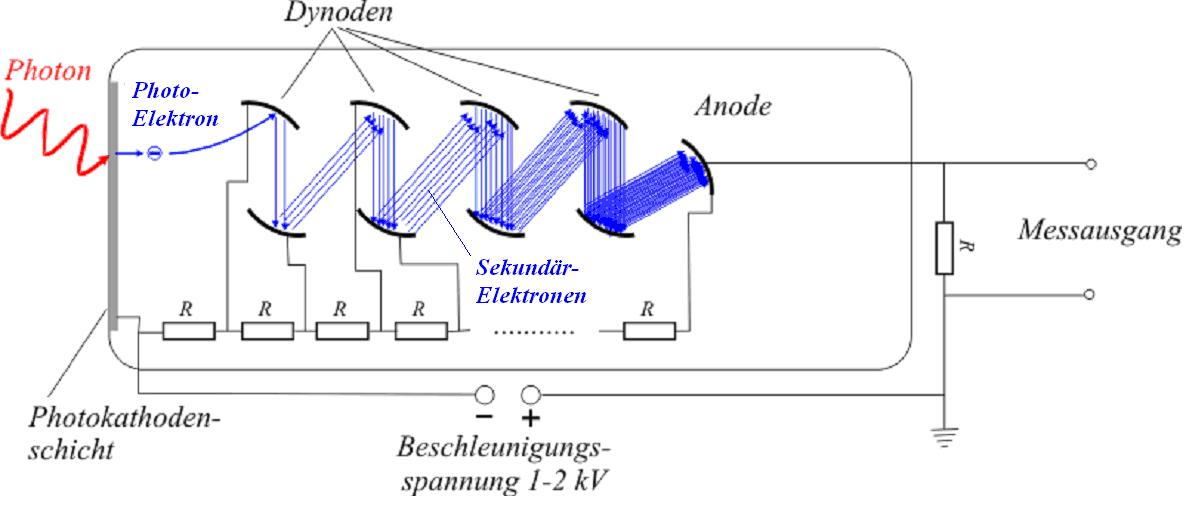
\includegraphics[width=0.8\textwidth]{Bilder/pmt.jpg}
        \caption{Veranschaulichung der Funktionsweise eines Photomultipliers. \cite{pmt}}
    \hfill
    \label{fig:d1}
\end{figure}
\noindent Ebenso bieten sich zur Rauschunterdrückung der Diskriminator und die 
Koinzidenzschaltung an. Der Diskriminator ist ein elektronisches Bauteil. Er 
lässt nur Spannungen oberhalb einer Schwelle passieren, alles darunter wird als 
Rauschen interpretiert und dementsprechend blockiert. Die Koinzidenzschaltung 
hat eine ähnliche Funktion. Sie lässt nur Signale durch, welche in einem 
bestimmten Zeitfenster quasi-simultan ankommen. Im konkreten Versuchsaufbau ist
die Koinzidenzschaltung das zentrale Element zur Unterdrückung von 
Untergrundereignissen. Ein Myon, das den Szintillatortank durchquert, erzeugt
entlang seiner Spur Lichtblitze, die von beiden Photomultipliern an den Enden
des Tanks detektiert werden. Da das Myon den Tank nahezu mit Lichtgeschwindigkeit
durchfliegt, treffen die Signale an beiden PMTs praktisch gleichzeitig ein. Die
Koinzidenzschaltung nutzt diese Eigenschaft aus, indem sie nur dann ein 
Ausgangssignal generiert, wenn beide PMTs innerhalb eines kurzen, einstellbaren
Zeitfensters einen Impuls liefern. Einzelne Impulse, die nur von einem PMT
stammen, etwa durch thermisches Rauschen oder Radioaktivität in der Umgebung,
werden hingegen verworfen. Dadurch wird sichergestellt, dass das auslösende 
Signal mit hoher Wahrscheinlichkeit von einem echten Myon stammt, welches den 
Detektors durchquert hat. \\
Für die Verarbeitung von Signalen müssen die Zeitinformationen für die weitere 
Analyse messbar gemacht werden. Diese übernehmen der Time-Amplitude-Converter 
(TAC) und der daran angeschlossene Vielkanalanalysator (MCA).
Der TAC ist im Wesentlichen ein elektronisches Bauteil, das eine Zeitdifferenz
in eine proportionale Spannungshöhe umwandelt. Im idealen TAC ist der Zusammenhang
zwischen dem Zeitinput und dem Amplitudenoutput linear \cite{tac}. Der 
Vielkanalanalysator (VKA oder MCA) ist ein digitales Messgerät, welches die 
eingehende Spannung in einen digitalen Kanalwert umwandelt und ein Histogramm 
erstellt. Für die Rückrechnun von den Kanälen in Zeiten wird ein 
Doppelimpulsintegrator genutzt. Dieser erzeugt zwei Pulse mit bekannten, 
einstellbaren Zeitabständen. Durch Vergleich mit dem TAC können folglich die 
Kanäle den Zeiten zugeordnet werden.


\subsection{Aufbau des Experiments}
\label{sec:d2}
Der schematische Aufbau des hiesigen Experiments ist in \autoref{fig:d2}
dargestellt. Zentrales Element ist der Szintillatortank (hier gefüllt mit einem 
Lösungsmittel), an den zwei Photomultiplier angeschlossen sind. Das hat den 
Zweck, die Lichtblitze, welche durch das Myon erzeugt werden, im späteren Verlauf 
von Hintergrundrauschen zu unterscheiden. Von den PMTs gehen die Signale durch 
eine Verzögerungsleitung und anschließend auf die Diskriminatoren, welche 
auf die Koinzidenzschaltung geschaltet sind. Diese Leitung gewährleistet eine 
zeitgleiche Detektion an der Koinzidenzschaltung, da die Signale der PMTs je 
nach Komponente und Leitungslänge unterschiedliche Laufzeiten haben können.
Nach der Koinzidenzschaltung wird ein Signal zunächst direkt auf ein Und-Gatter 
geschaltet, welches das Start-Signal an den TAC weiterleitet. Das weitere 
Signal, welches auf das Und-Gatter geht, kommt aus dem Monoflop, dieses ist 
entscheidend, ob die Messung startet, da die Myonendetektion nicht alleinig 
reicht, es muss auch ein Zerfall gemessen werden. Das Monoflop wird durch das
erste Koinzidenzsignal mit einer Verzögerung von $\qty{30}{\nano\second}$
ausgelöst. Die Verzögerung stellt sicher, dass der Startimpuls den TAC 
erreicht, bevor die Logik umgeschaltet wird. Die Suchzeit $T_s$ des Monoflops 
ist dabei entscheidend für die Genauigkeit der Messung, sie definiert das
Zeitfenster, in dem die Elektronik auf den Zerfall des zuvor detektierten Myons
wartet. Anschließend liefert das Monoflop sowohl einen normalen als auch einen
invertierten Ausgang. Der invertierte Ausgang sperrt über das erste Und-Gatter
weitere Startsignale, sodass ausschließlich die erste Koinzidenz den TAC startet.
Gleichzeitig gibt der normale Ausgang über das zweite Und-Gatter den Stop-Eingang
frei. Erst wenn nun eine weitere Koinzidenz auftritt, wird ein Stop-Signal erzeugt
und an den TAC weitergeleitet. Hinter beiden Gattern befinden sich Impulszähler,
diese leiten die Signale an den TAC weiter, welcher Spannungen an den MCA und
den Computer weitergibt, wo die Daten gesammelt und in Form von Histogrammen 
gespeichert werden.
\vspace{0.5em} \\
\noindent Der Doppelimpulsintegrator über der Koinzidenzschaltung dient 
lediglich der Kalibierung des TAC. Er erzeugt zwei Pulse mit bekannten 
Zeitabständen, sodass die Kanäle des MCA den Zeiten zugeordnet werden können.
\begin{figure}[H]
    \centering
        \centering
        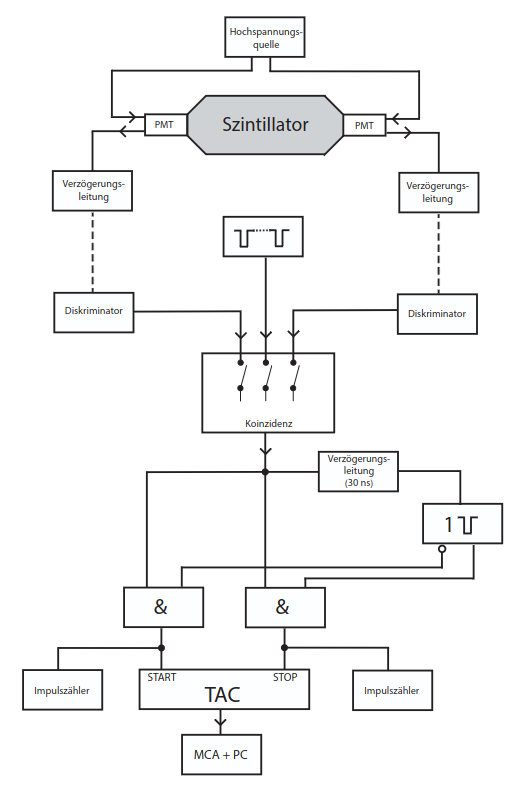
\includegraphics[width=0.85\textwidth]{Bilder/schaltplan.png}
        \caption{Schaltbild zum Experiment \cite{anleitung16}.}
    \hfill
    \label{fig:d2}
\end{figure}
\noindent Der reale Aufbau ist in \autoref{fig:d3} zu sehen. Oben ist der 
Szintillatortank mit den beiden PMTs zu erkennen, darunter die befindliche 
Schaltungstechnik.
\begin{figure}[H]
    \centering
        \centering
        
\includegraphics[width=0.85\textwidth]{Bilder/aufbau.jpg}
        \caption{Aufbau des Versuchs (Eigenaufnahme).}
    \hfill
    \label{fig:d3}
\end{figure}


\subsection{Messvorgang}
\label{sec:d3}
Als allererstes werden die PMTs auf ihre Funktion geprüft, das geschieht über 
eine Probe mithilfe eines Oszilloskops. Im nächsten Schritt werden die Schwellspannungen der Diskriminatoren 
eingestellt. Dazu wird ein Impulszähler an den Ausgang jedes Diskriminators 
angeschlossen. Die Schwellspannung wird so gewählt, dass an beiden Ausgängen
eine Zählrate von etwa $\qty{30}{s^{-1}}$ gemessen wird. Gleichzeitig wird die
Pulsdauer der Diskriminatorausgänge auf $\qty{10}{\nano\second}$ festgelegt.
Diese Einstellung verhindert Doppeltriggerungen durch einen einzelnen Lichtblitz
und stellt die zeitliche Präzision für die nachfolgende Koinzidenzschaltung 
sicher. Nun wird ein Oszilloskop an den Ausgang des Monoflops angeschlossen, 
um die Suchzeit $T_s$ einzustellen. Anschließend wird die Schaltung bis zum
TAC vervollständigt und dessen Funktionsweise überprüft. Dazu wird der
Doppelimpulsgenerator anstelle der PMTs an die Koinzidenzschaltung angeschlossen
und der Messbereich des TAC an die Suchzeit $T_s$ angepasst. Zuletzt wird der
Vielkanalanalysator kalibriert. Hierzu werden mit dem Doppelimpulsgenerator 
Impulse mit verschiedenen Zeitdifferenzen im Bereich von $\qty{0,3}{\micro\second}$
bis $\qty{9,9}{\micro\second}$ erzeugt und die zugehörigen Kanäle des MCA notiert.
Aus diesen Messwerten wird eine Kalibrationsgerade für den Zusammenhang 
zwischen Kanalnummer und Zeitdifferenz bestimmt. Die Messung zur Erfassung der 
Daten für die Lebensdauer der Myonen beginnt und läuft über vier Tage.
